\documentclass[10pt,a5paper,twoside]{book}
\usepackage[utf8]{inputenc}
\usepackage[czech]{babel}
\usepackage[T1]{fontenc}
\usepackage{amsmath}
\usepackage{amsfonts}
\usepackage{amssymb}
\usepackage{hyperref}
\usepackage[dvips]{graphicx}
\usepackage[top=2cm, left=1.5cm, bottom=1.5cm, includefoot]{geometry}
\usepackage{eso-pic}
\usepackage{pdfpages}
\usepackage{textpos}
\usepackage{titlesec}
\usepackage{verbatim}
\fontencoding{T1}
\fontfamily{cmss}
\fontseries{m}
\fontshape{n}
\setlength{\belowcaptionskip}{-15pt} % mezera za popiskem obrázku
\usepackage{xcolor}
\usepackage{pdfpages}
% pdftk TitlePage14_1.pdf Jihacas14_1.pdf cat output Jihocas_14_1-WEB_kontrola.pdf spojeni pdf

\titleformat{\section}
{\color{blue}\normalfont\Large\bfseries}
{\color{blue}\thesection}{1.2em}{}

\newcommand{\autor}[1]{
	\begin{flushright}
	\textit{#1}
	\end{flushright}
}

\begin{document} 

%\begin{titlepage}
\begin{center}

% Upper part of the page. The '~' is needed because \\
% only works if a paragraph has started.
\includegraphics[width=0.15\textwidth]{./logo}~\\[1cm]

\textsc{\LARGE University of Beer}\\[1.5cm]

\textsc{\Large Final year project}\\[0.5cm]

% Title
\HRule \\[0.4cm]
{ \huge \bfseries Lager brewing techniques \\[0.4cm] }

\HRule \\[1.5cm]

% Author and supervisor
\begin{minipage}{0.4\textwidth}
\begin{flushleft} \large
\emph{Author:}\\
John \textsc{Smith}
\end{flushleft}
\end{minipage}
\begin{minipage}{0.4\textwidth}
\begin{flushright} \large
\emph{Supervisor:} \\
Dr.~Mark \textsc{Brown}
\end{flushright}
\end{minipage}

\vfill

% Bottom of the page
{\large \today}

\end{center}
\end{titlepage}



\section*{K obrázku na titulní straně}
Robotický dalekohled BOOTES2. Experimentální stanice La Mayora nedaleko Málagy. Průměr primárního zrcadla 60 cm; systém Ritchey-Chretien.
\vfill
\section*{JihoČAS}
Vydává: Jihočeská pobočka České astronomické společnosti.\\
Redakce a adresa pro zasílání příspěvků: Martin Kákona, U Jatek 19/III, 392 01 Soběslav, e-mail: \href{mailto:martin.kakona@astro.cz}{martin.kakona@astro.cz}.\\
Sazba: Roman Dvořák, e-mail: \href{mailto:roman-dvorak@email.cz}{roman-dvorak@email.cz}.\\
Vytisknuto s laskavým přispěním Jednoty České Budějovice.\newpage


\section*{Nový vzhled JihoČASu}
První letošní číslo JihoČASu vychází až nyní z mnoha důvodů. Jednak jsem začátkem roku nebyl v republice a pak je tu mnohem závažnější důvod – snažíme se přejít na jiný systém sazby. Tento přechod není úplně bezbolestný a zatím se rozhodně nejedná o usnadnění práce ;)
Doufáme, že se vám nová grafická úprava JihoČASu bude líbit, respektive, že pro vás nebude tak odpudivá, abyste mohli i nadále z JihoČASu čerpat informace.

\begin{flushright}
Martin Kákona
\end{flushright}
\newpage

\section*{V únoru bez novu}
\autor{Milan Blažek,\\ Hvězdárna a planetárium hl. m. Prahy, p. o.}

Měsíční fáze jsou nejnápadnějším důkazem obíhání Měsíce kolem Země. Jelikož Měsíc nesvítí svým vlastním světlem, vidíme z k nám přivrácené polokoule Měsíce jen tu část, která je osvětlena naší nejbližší hvězdou – Sluncem. Podle toho, jak velký je úhel mezi směry Země – Slunce a Země – Měsíc, můžeme sledovat pouze určitou část Měsíce, podle toho v jakém směru se nachází Měsíc na obloze vzhledem ke Slunci. Tyto změny vzhledu nazýváme fáze a vyjadřujeme je nejčastěji ve dnech (případně dnech a jeho desetinách), které uplynuly od novoluní (novu). 

V novu není Měsíc ze Země pozorovatelný, neboť Slunce osvětluje odvrácenou polokouli našeho vesmírného souseda. I tak ale máme možnost s úžasem sledovat tuto fázi Měsíce na vlastní oči. Ve vzácných případech Měsíc zakryje Slunce a nastává zatmění Slunce. Tou dobou je náš kosmický souputník právě v novu.   

Měsíční novy po sobě následují v periodě 29,5 dne. Mezi tím se vystřídají všechny měsíční fáze. Tomuto cyklu odborně říkáme synodický měsíc nebo lunace.

Číslování lunací, se kterým se můžeme setkat v různých astronomických ročenkách apod., bylo zavedeno počínaje novem číslo 1, který nastal 17. ledna roku 1923. Jubilejní lunace číslo 1000 tak připadla na 23. října 2003. V únoru 2014 tedy evidujeme lunaci číslo 1127.

Únor je nejkratším kalendářním měsícem. Vždy po 19 letech tak nastává zajímavá situace. V lednu a březnu se vyskytují dva novy, zatímco v únoru nemáme žádný. Už jste si toho v kalendáři nebo hvězdářské ročence všimli? :-)

Tato událost většinu z nás potkala v roce 1995 a přeji nám všem, abychom ve zdraví byli svědky i té následující v únoru 2033.

\section*{Kresby Měsíce podle fotografií}
\autor{Milan Blažek,\\Hvězdárna a planetárium hl. m. Prahy, p. o.}

Poslední dobou jsou po mně žádány především kresby překreslené z fotografií předních světových astrofotografů. Při dnešních technických možnostech pozorovatelů se na snímcích zobrazují úchvatné podrobnosti, jaké okem u dalekohledu stěží zpozorujeme. Detaily na kvalitních fotografiích bývají tak jemné, že se při zakreslování obtížně reprodukují. Nejtenčí hrot fixu má sice průměr pouhých 0,5 mm, i tak ale vytvoří tečku o určité plošce. Pokud chceme detail nakreslit věrohodně ve stejné velikosti, jako na předlohové fotografii, dostáváme se do problému s místem. Tuto situaci lze řešit tím, že fotografii vytiskneme velkou, čímž získáme více prostoru pro zakreslování v poměru 1:1. To je sice prima, ale pak se zase dostáváme do problému s časem, který vystínování tak velké plochy zabere. Já nyní kreslím na formát A4 a zhotovení jedné kresby mi zabere 100 – 200 hodin čistého času. Pro mne osobně je to problém, neboť kresbu většinou potřebuji dokončit do určitého termínu (uzávěrka časopisu atp.). Abych vše stihl, jsem „nucen“ kreslit průměrně dvě až tři hodiny denně! Kde na to brát čas - v dnešní uspěchané době?! S trochou nadsázky mohu napsat, že ani nevím, co je televize. Kromě překreslování fotografií se snažím aktivně amatérsky pozorovat a dělat zákresy přímo z vizuálního sledování dalekohledem. Pro amatérského astronoma mají právě tyto kresby větší hodnotu, ale u laika se již takovému zájmu netěší, neboť nevypadají tak úchvatně. Podle mne jsou kresby z fotografií spíše uměleckým dílem… 
\begin{figure}[htbp]
\centering
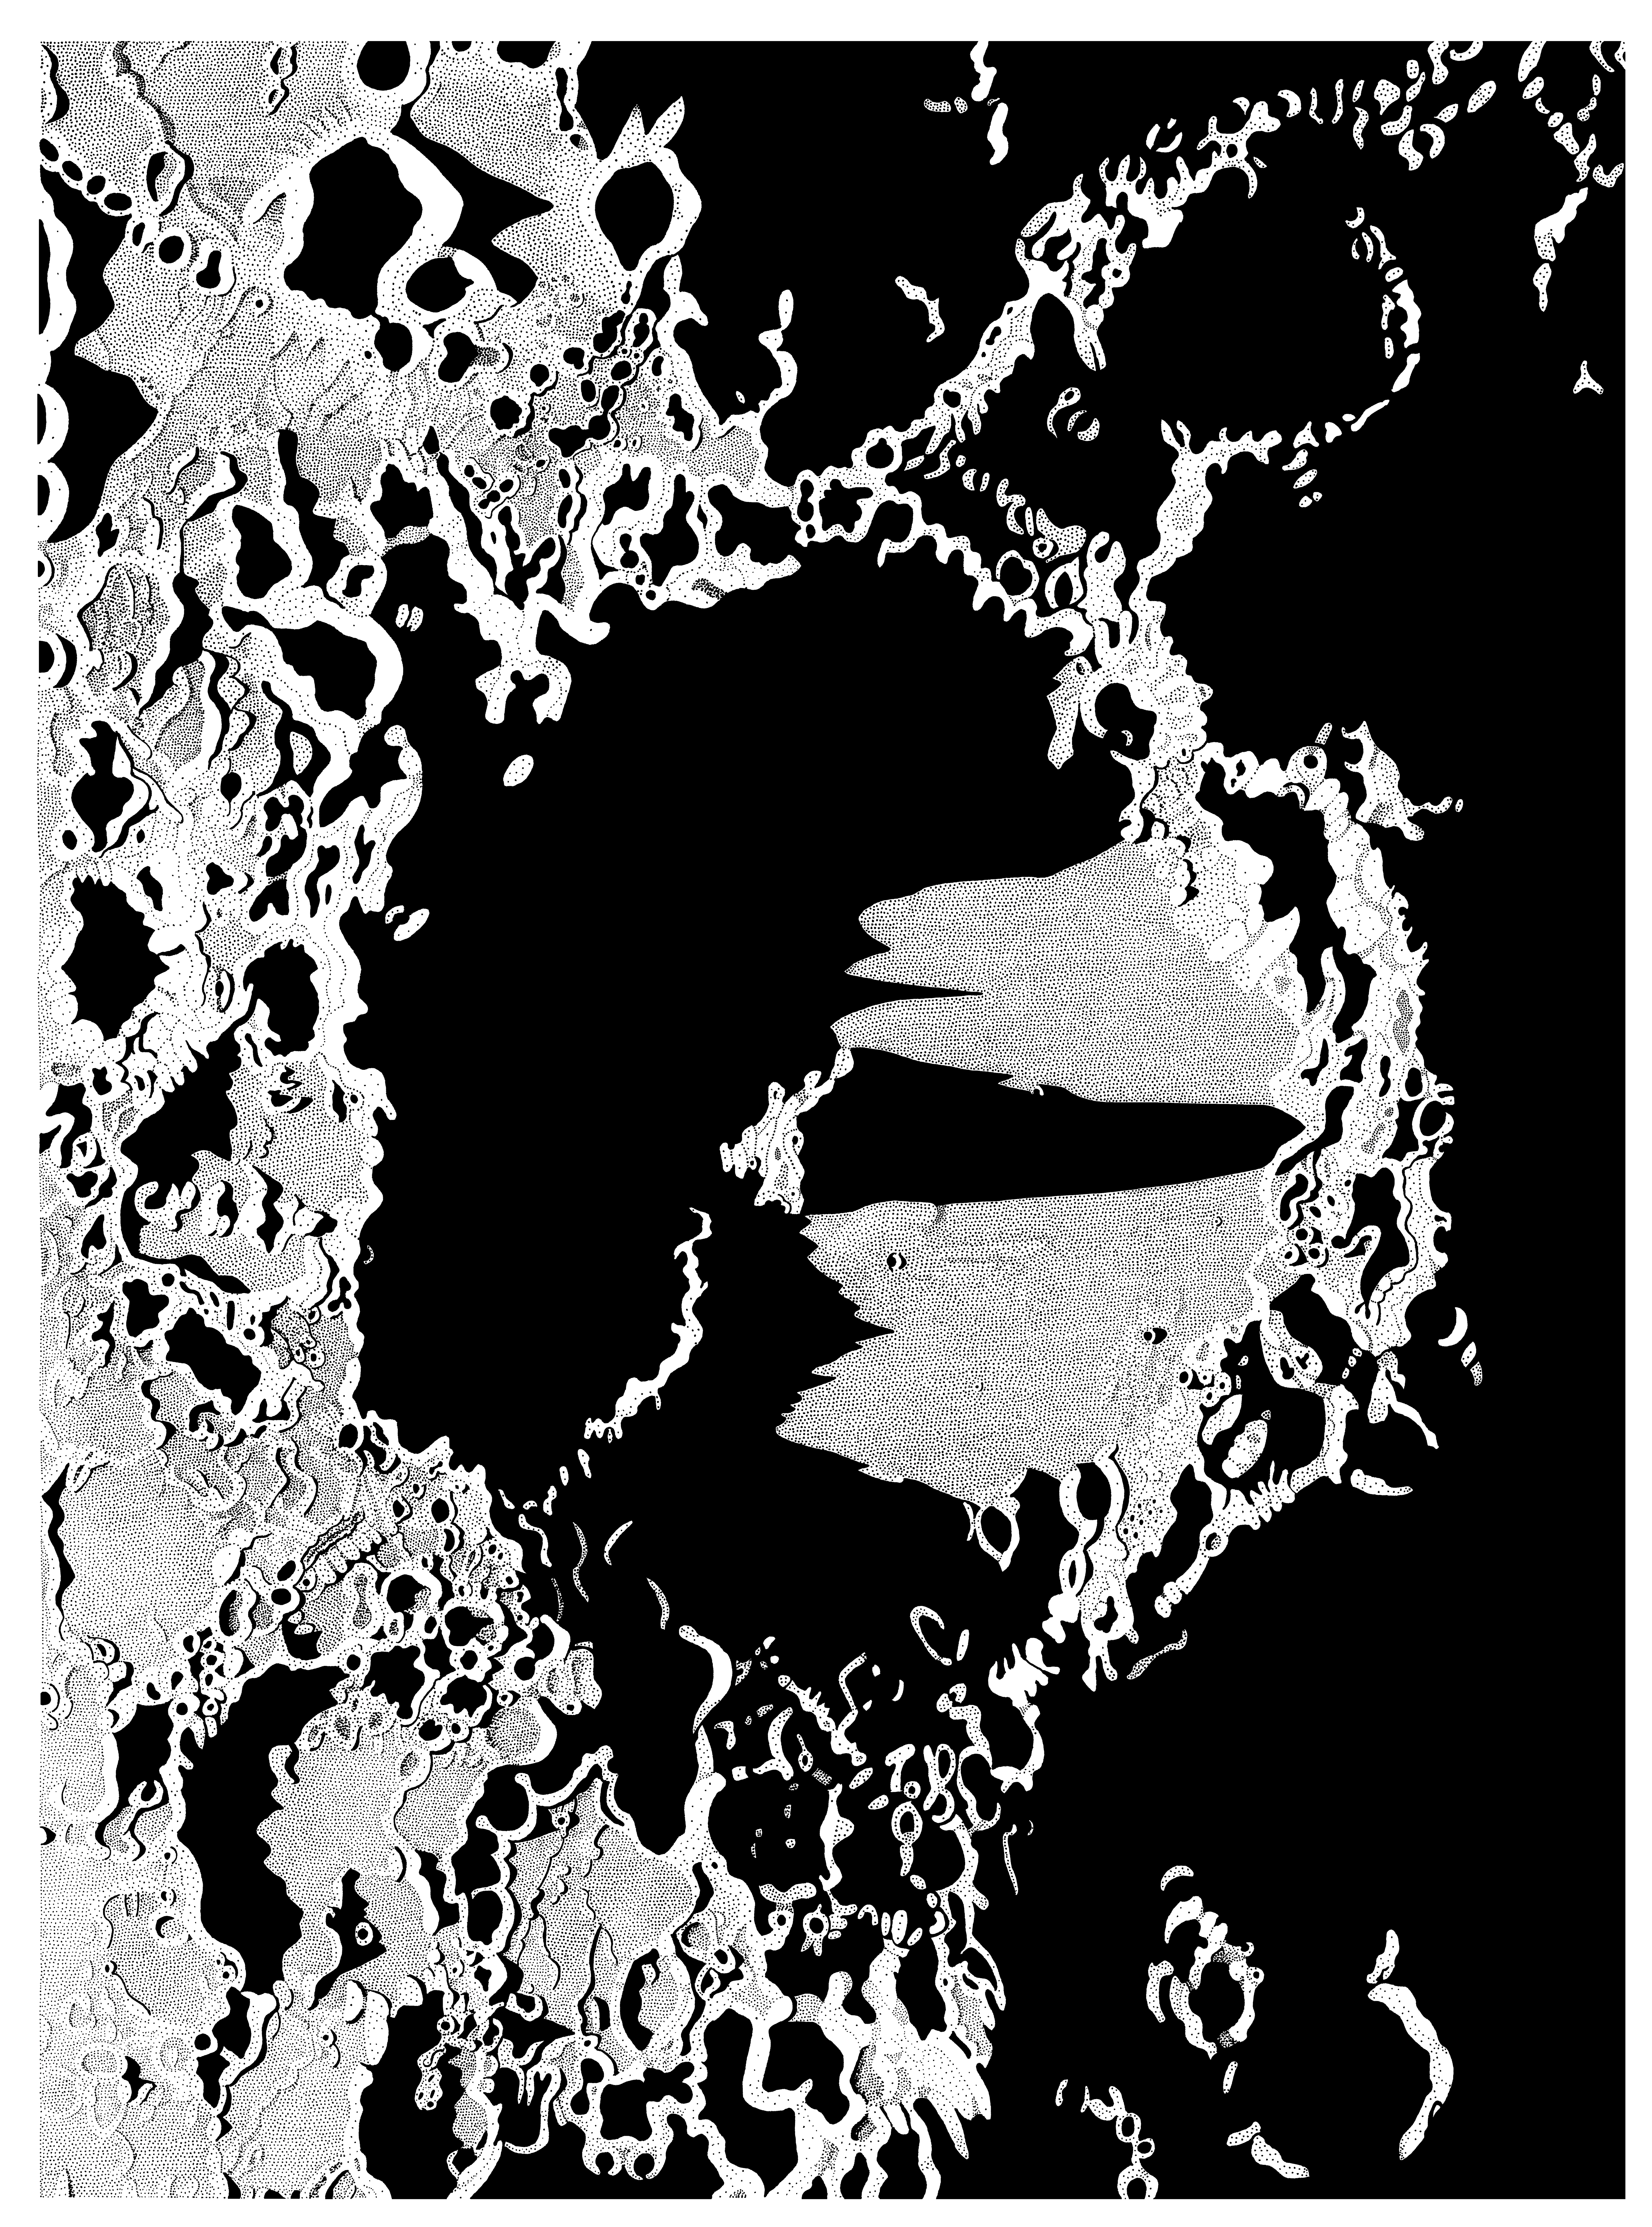
\includegraphics[width=5cm]{blazek2/Albategnius_original.eps}
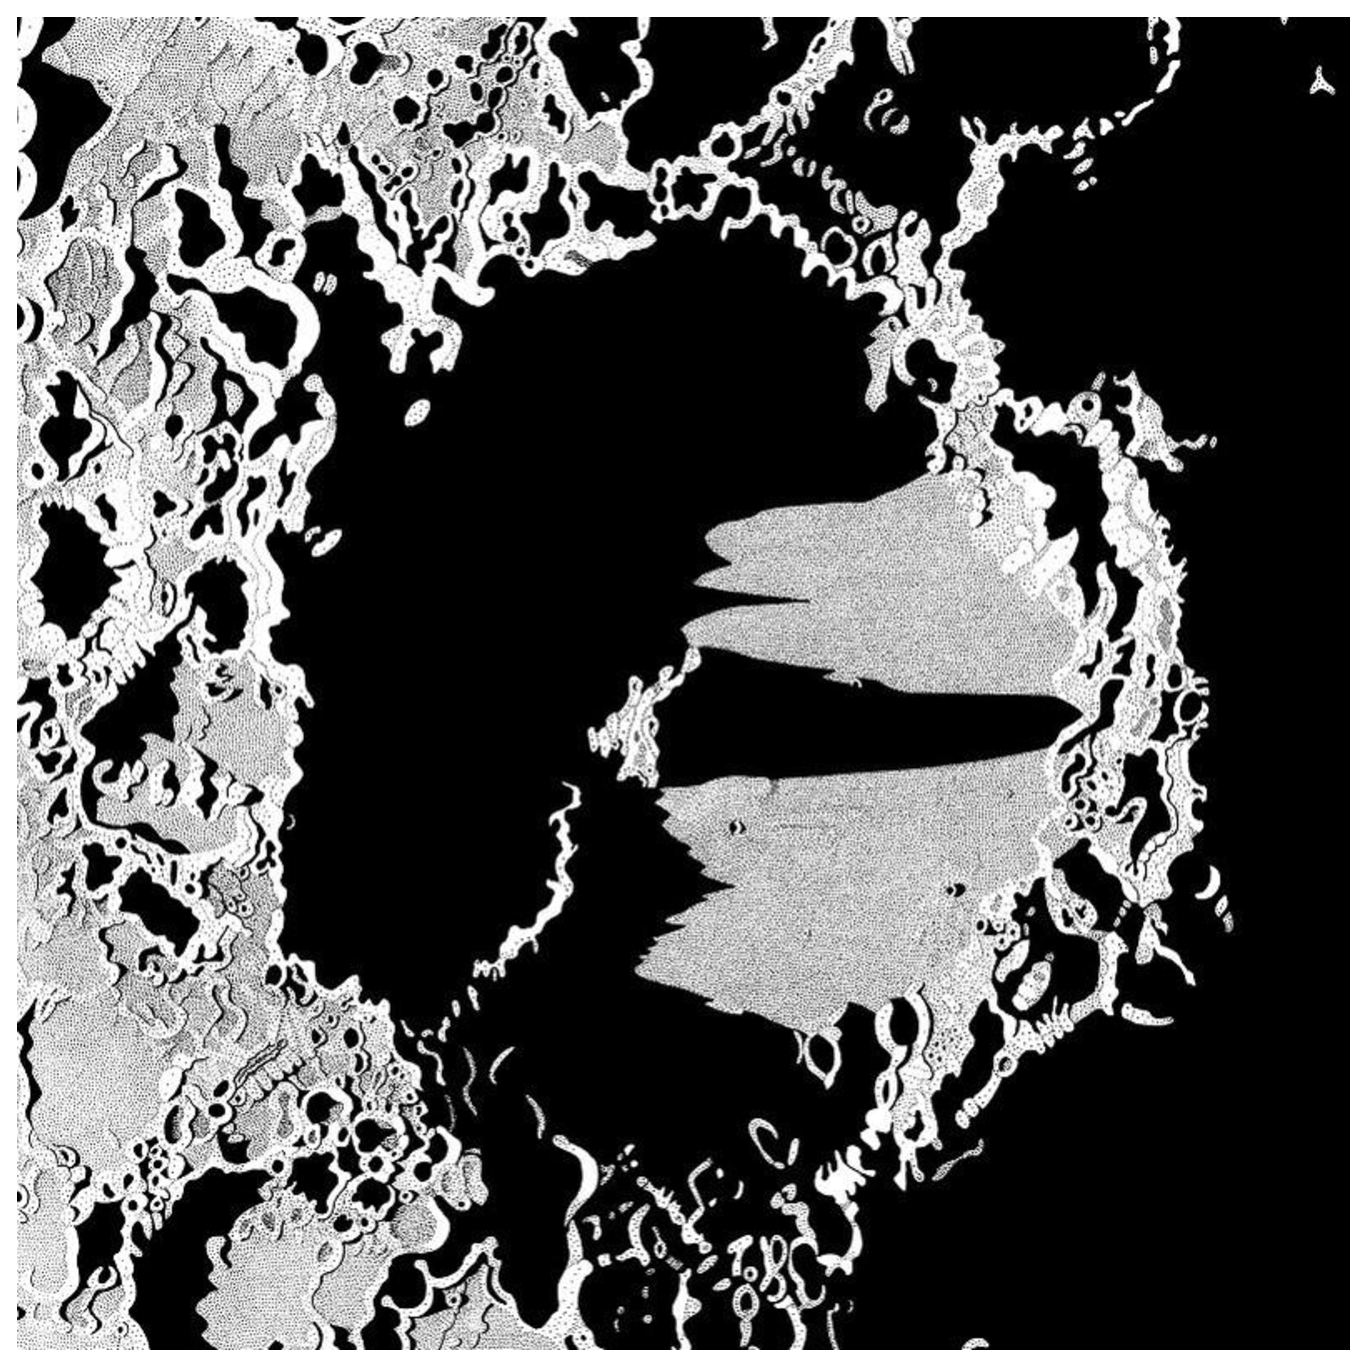
\includegraphics[width=5cm]{blazek2/Albategnius_z_galerie.eps}\\
Pro tištěnou verzi JihoČASu předkládám ukázku poslední vložené kresby do galerie v době odeslání článku redakci (čtvercová kresba) a původní zákres (obdélníková kresba).
\end{figure} 

Bohužel (nebo snad bohudík?) právě o takové kresby je docela zájem. Nedávno mne oslovil Andrew Bray z Austrálie, jehož fotografii jsem překresloval, že by rád umístil mé skici na jeho stránkách. Těžko předvídat, do jaké míry bude stránka aktualizována v době, kdy JihoČAS vyjde. Zatím je můj příspěvek na této stránce omezený a probíhají na něm prvotní úpravy. I tak ale posílám čtenářům odkaz na zkušební verzi: \url{http://www.visit-the-moon.com/milan-blazek-ink-drawings}.



\section*{Pozorování meteorů za každého počasí}
\autor{\href{mailto:martin.kakona@astro.cz}{Martin Kákona},\\Jihočeská pobočka ČAS}

Už se vám určitě někdy stalo, že jste chtěli pozorovat maximum meteorického roje a bylo zataženo. Nebo svítil Měsíc, takže z předpovídaných 30 meteorů za hodinu jste viděli 4 nebo žádný a ještě jste třeba zmokli. Bohužel, to je realita pozorovatelů meteorů už po desítky let. Dnešní technika ale umožňuje se těmto starostem úplně vyhnout.

V tomto článku vám chceme představit metodu pozorování meteorů, která je nezávislá na počasí, Měsíci či denní době. Dokonce můžete pozorovat doma v teple u kamen, pokud si vhodně umístíte počítač ;-) Jedná se o radiové pozorování meteorů metodou dopředného odrazu.
\begin{figure}[htbp]
	\begin{center}
		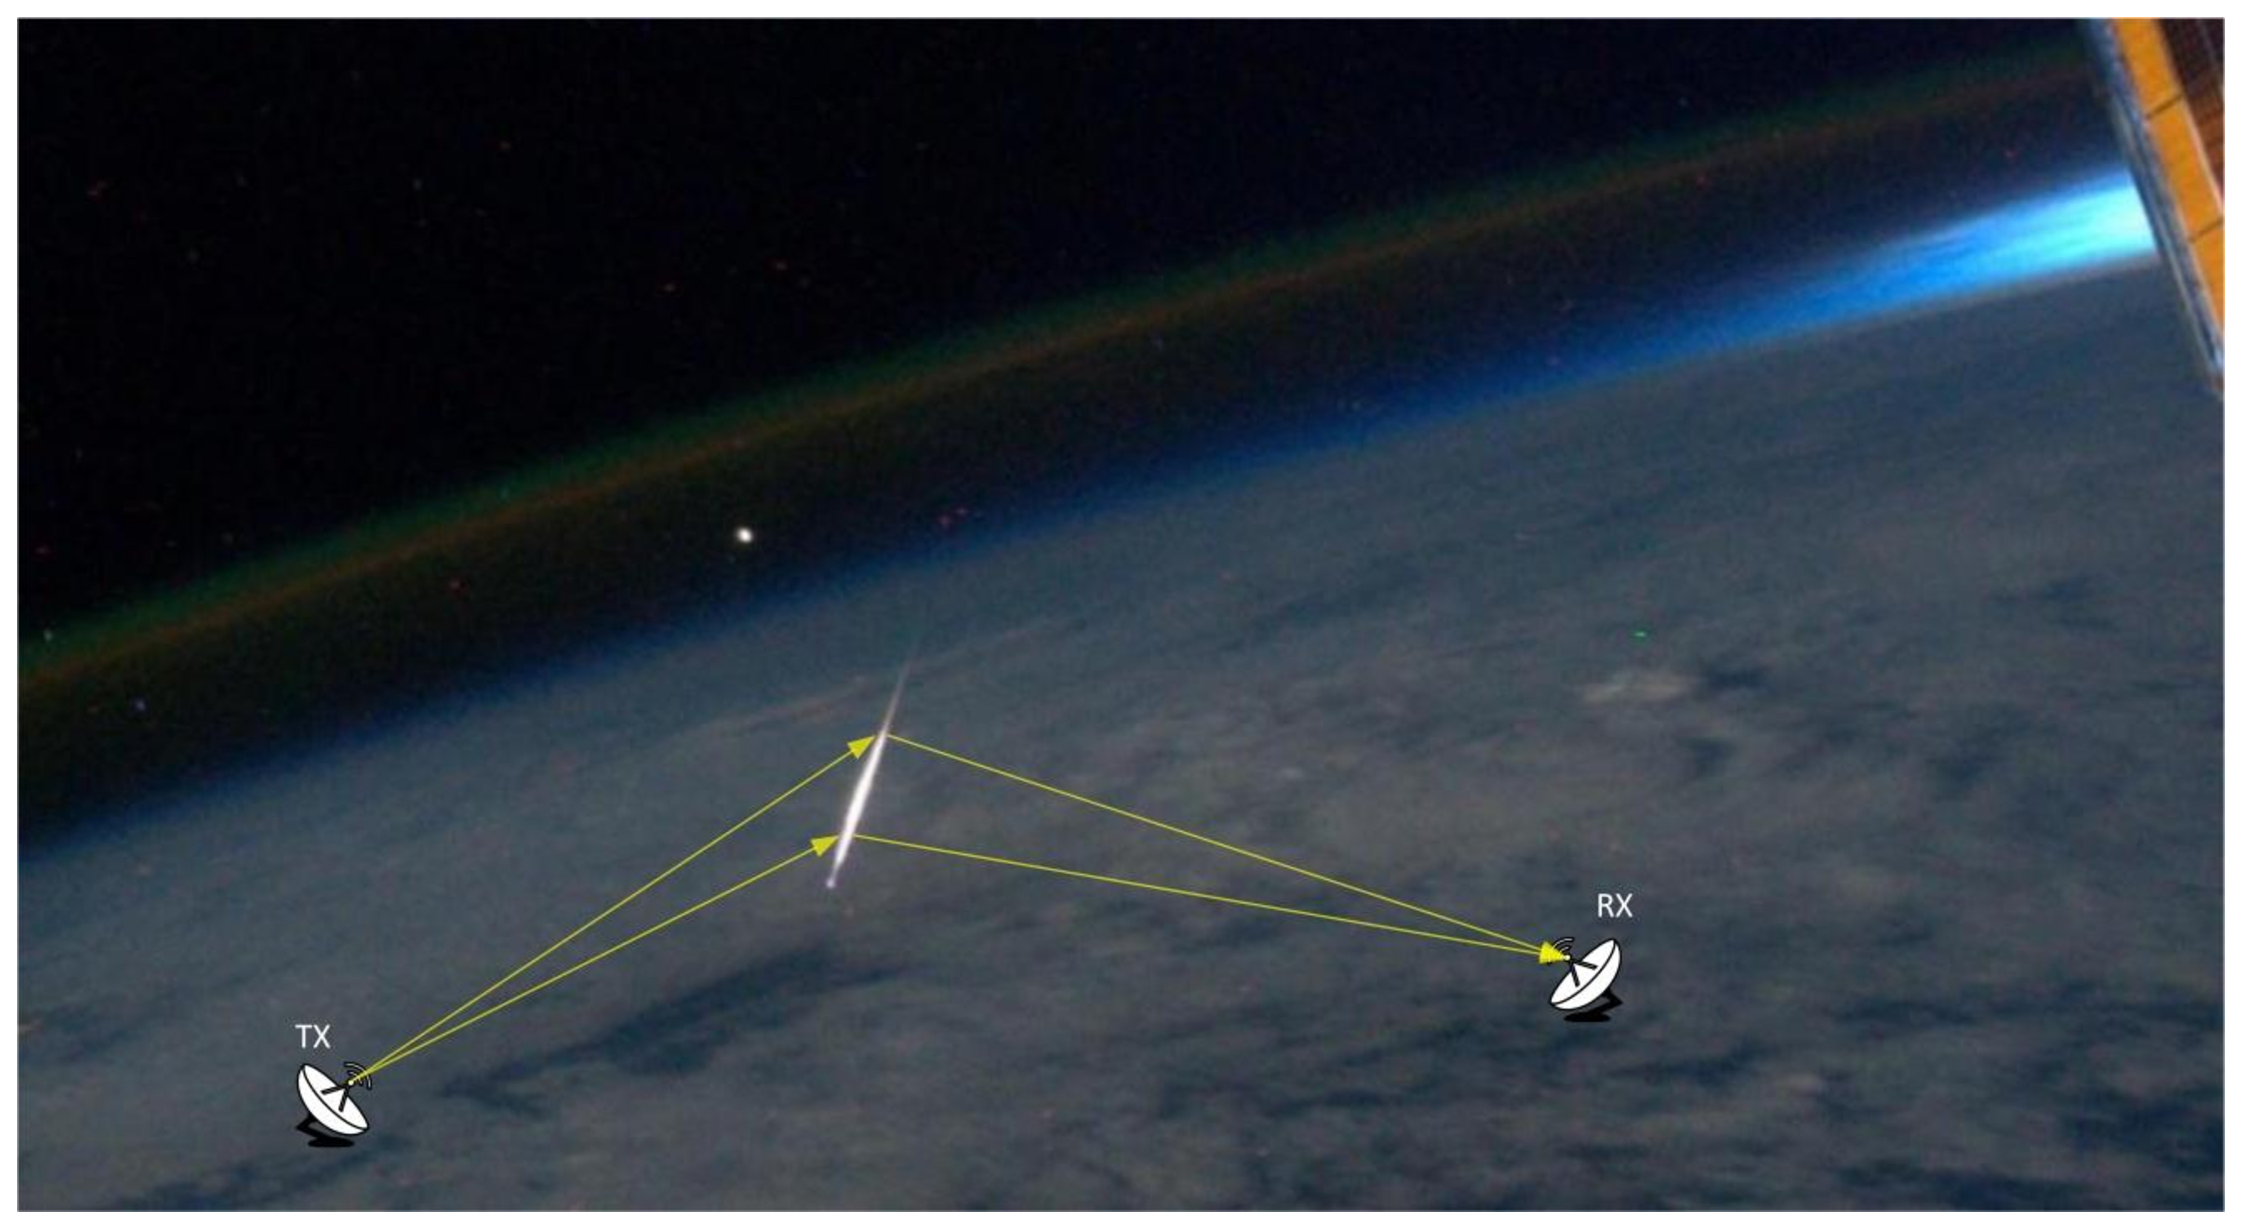
\includegraphics[width=9cm]{graves/graves_soubory/image001.eps}
	  	\caption{Princip radiové detekční metody forward scattering.}
	  	\label{fig:}
	\end{center}
\end{figure}
Podkladový obrázek vyfotil astronaut Ron Garan (NASA) z ISS.
Princip metody, který je znázorněn na Obr. 1, je velmi jednoduchý. Na povrchu Země jsou umístěny vysílač (TX) a přijímač (RX) ve velké vzdálenosti (stovky kilometrů) od sebe tak, že jsou jejich antény nasměrovány nahoru na oblohu a za normálního stavu se „neslyší“. Pokud atmosférou mezi vysílačem a přijímačem proletí meteoroid, vytvoří meteor, tedy meteorickou stopu (typicky ve výšce 80 až 100 km nad zemí), která je tvořena převážně ionizovaným plynem. Vzhledem k tomu, že ionizovaný plyn je vodivý, je to podobné, jako kdybyste zavěsili do prostoru na chvíli vodivý plech. Stopa funguje podobně jako zrcadlo a radiová vlna z vysílače (TX) se od stopy odrazí. Odraz pak zachytí přijímací anténa (RX). Odraz je možné pozorovat tak dlouho, dokud ionizovaný plyn tzv. nerekombinuje a neztratí svoji vodivost.

Tato metoda pozorování není nová. Na Zemi existuje mnoho stanic, které v minulosti touto metodou pozorovaly a stále pozorují, například stanice umístěná na hvězdárně ve Vsetíně. K pozorování se využívá rozhlasové vysílání na krátkých vlnách nebo televizní vysílače v prvním televizním pásmu. V současnosti ale ubývá stanic na těchto kmitočtech. U rozhlasového vysílání se přechází na vyšší kmitočty, které umožňují kvalitnější přenos, ovšem na kratší vzdálenosti a televizní vysílání opouští nižší kmitočty současně s digitalizací. Přitom vyšší kmitočty nejsou pro pozorování meteorů moc vhodné, protože čím vyšší kmitočet použijeme, tím větší ionizační hustotu musí mít plyn tvořící stopu, aby došlo k odrazu o stejné intenzitě, tedy meteoroid musí mít větší energii. 
 
Naštěstí se v Evropě objevil vysílač, který je pro dané pozorování velice vhodný. Je to zařízení francouzské armády s označením \href{http://en.wikipedia.org/wiki/Graves_\%28system\%29}{GRAVES}. Tento radar slouží k určování drah družic. Vysílací anténa je umístěna na zrušeném vojenském letišti na souřadnicích $47,3480^{\circ}$ severní šířky a $5,5151^{\circ}$ východní délky. Vysílá směrem na jih s vyzařovacím úhlem ve vodorovné rovině $180^{\circ}$.
\begin{figure}[htbp]
	\begin{center}
		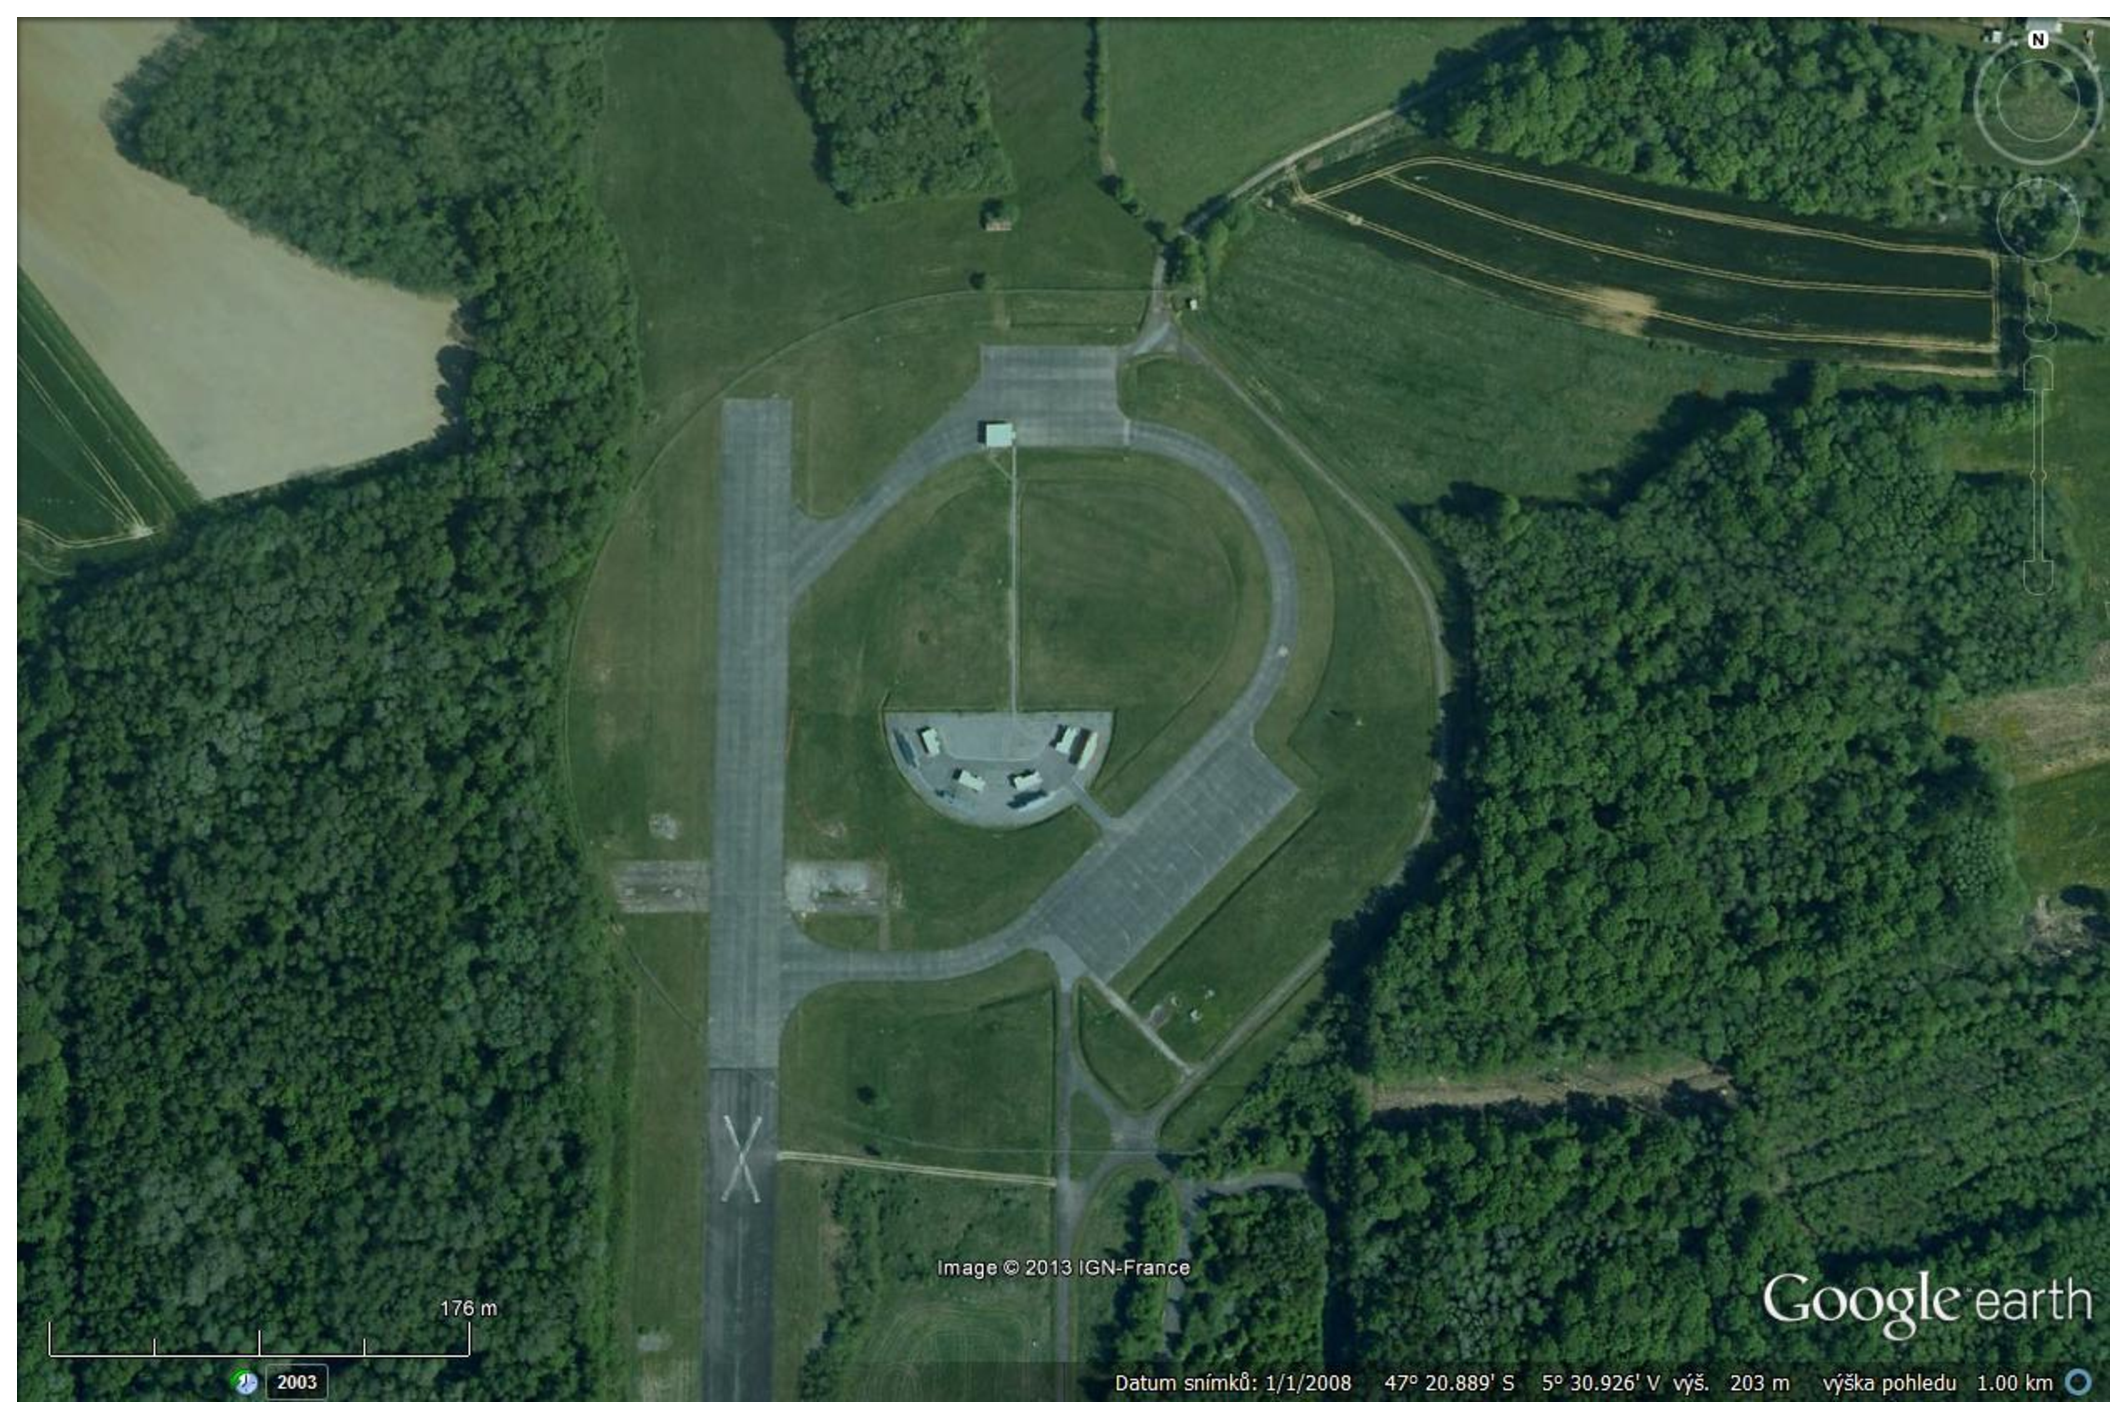
\includegraphics[width=8cm]{graves/graves_soubory/image002.eps}
	  	\caption{Letecký pohled na vysílací antény radaru GRAVES. Nalevo je vidět zrušená dráha letiště. Čtyři vysílací antény jsou vidět v půlkruhu uprostřed.}
	  	\label{fig:}
	\end{center}
\end{figure}
Radar GRAVES není zcela ideální zdroj signálu pro Českou republiku, protože nevysílá naším směrem, ale meteory které ozáří, jsou přesto detekovatelné přijímačem umístěným na našem území. Pouze je třeba říct, že pokud použijeme jako zdroj signálu GRAVES, „uvidíme“ většinou meteory nízko nad jižním obzorem někde v oblasti Alp, tedy meteory, které budou jen těžko pozorovatelné od nás vizuálně. Tento nedostatek je ale více než vyvážen faktem, že GRAVES vysílá opravdu velkým výkonem. Hovoří se o jednotkách megawattů. Přesný výkon není znám – jak jsme již psali, jedná se o vojenské zařízení.

Díky obrovskému vysílacímu výkonu můžeme pro příjem signálů odražených od meteorů použít velmi jednoduché zařízení s ne příliš rozměrnou anténou. V podstatě se dá říci, že můžete klidně pozorovat meteory ve městě třeba z balkónu paneláku (pokud ovšem váš soused neprovozuje výrobky označené \href{http://en.wikipedia.org/wiki/File:Comparison_of_two_used_CE_marks.svg}{nesprávným logem}).
\begin{figure}[htbp]
	\begin{center}
		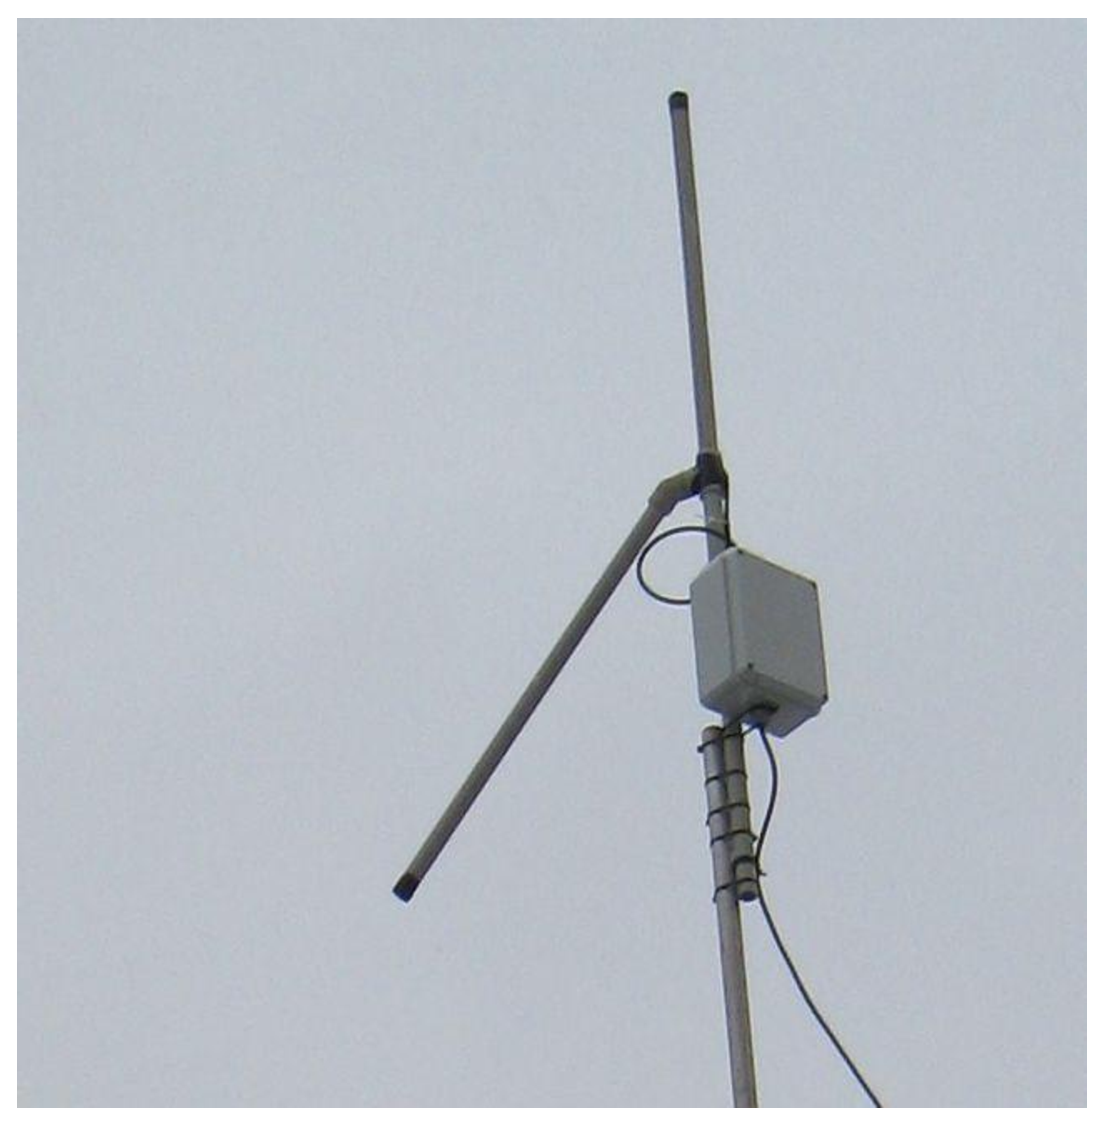
\includegraphics[width=7cm]{graves/graves_soubory/image005.eps}
	  	\caption{Možná konstrukce přijímací antény.}
	  	\label{fig:}
	\end{center}
\end{figure}
Anténa může být opravdu jednoduchá. Na Obr. 3 je příklad antény, kterou si svařili z plastových vodovodních trubek na Hvězdárně ve Vyškově. Pro představu, délky trubek jsou 0,5 m.

Také přijímač dnes nemusí být drahý. Vhodné je použít takzvaný softwarově definovaný přijímač (Software Defined Radio - SDR). Jedná se o zařízení, ve kterém je signál nejdříve transformován na kmitočet, který umíme převést analogově digitálním převodníkem na data, a veškeré další zpracování se již děje digitálně, tedy žádné cívky, žádné laděné obvody a podobně. Pokud signál vysílače převedeme na dostatečně nízký kmitočet, můžeme jako analogově digitální převodník použít třeba zvukovou kartu počítače a celý zbytek rádia nám obstará speciální program, který máme na počítači spuštěný.

Dále popíši zařízení, které používáme pro příjem meteorů na \href{http://www.astrozor.cz/index.php?udalost=5}{Svákovské hvězdárně} v Soběslavi. Speciálně pro tento účel jsme vyvinuli otevřený hardware, který je plně zdokumentován na webu \url{http://www.mlab.cz/} . Na uvedeném webu naleznete schémata zapojení, výrobní podklady pro výrobu desek plošných spojů a i potřebný software pro realizaci celé přijímací stanice. Výhoda tohoto řešení je v tom, že je modulární, založené na open source stavebnici MLAB a lze ho tedy v budoucnu rozšiřovat a stále metodu sledování zlepšovat. Záleží pouze na invenci pozorovatelů.
\begin{figure}[htbp]
	\begin{center}
		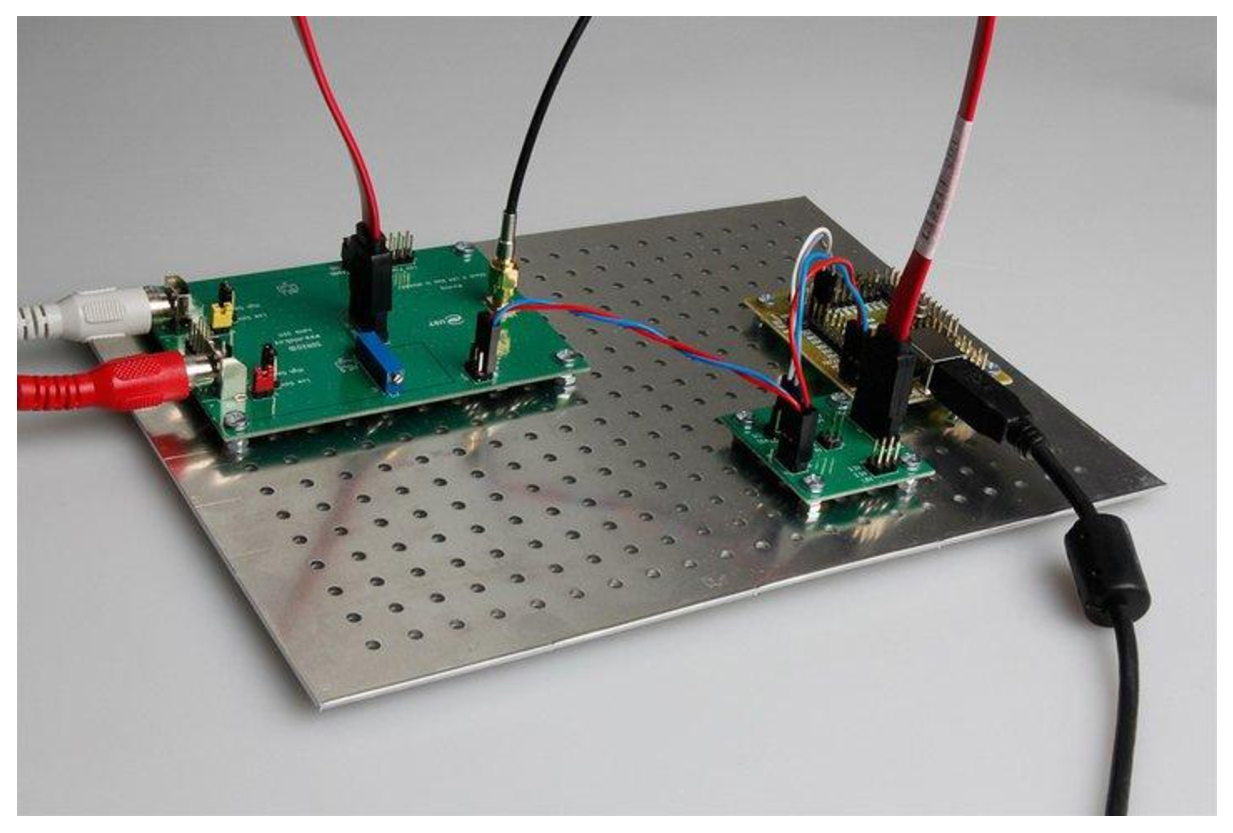
\includegraphics[width=8cm]{graves/graves_soubory/image006.eps}
	  	\caption{Radiová Meteorická Detekční Stanice RMDS01A založená na Softwarově definovaném přijímač SDRX01B.}
	  	\label{fig:}
	\end{center}
\end{figure}
Tak tedy detekční stanice, které říkáme \href{http://wiki.mlab.cz/doku.php?id=cs:rmds}{RMDS01A} se skládá z již výše zmíněné antény typu \href{http://www.ccars.org/projects/2mgp/tech_2mgp.htm}{$\frac{1}{4}\lambda$ GP}. Dále z nízkošumového anténního předzesilovače \href{http://wiki.mlab.cz/doku.php?id=cs:lna}{LNA01A}, který při použití takto jednoduché antény poskytuje dostatečný zisk i pro pozorování slabých meteorů. Ze softwarově definovaného přijímače \href{http://wiki.mlab.cz/doku.php?id=cs:sdrx}{SDRX01B} a z oscilátoru \href{http://www.mlab.cz/Modules/Clock/CLKGEN01B/DOC/CLKGEN01B.cs.pdf}{CLKGEN01B}. Dále je zapotřebí už jen PC se zvukovou kartou, která umí vzorkovat stereofonní signál s rychlostí alespoň 48 ks/s a vhodný software. My používáme volně šiřitelný program \href{http://www.qsl.net/dl4yhf/spectra1.html}{Spectrum Lab}, který jsme opatřili vlastním \href{http://www.mlab.cz/WebSVN/filedetails.php?repname=MLAB&path=\%2FDesigns\%2FMeasuring_instruments\%2FRMDS01A\%2Fusr\%2FSVAK1_.txt}{skriptem} na detekci meteorů. Takže přijímač detekuje meteory zcela automaticky, o každém meteoru udělá záznam o síle odrazu, délce trvání stopy a podobně. Zároveň u meteorů, u kterých trvá radiový dosvit stopy déle než 2,5 s, program pořídí audiozáznam, který je možné později analyzovat.

No a co je možné takovým rádiem „vidět“ a vlastně i slyšet? Především, když rádio zprovozníte, zarazí vás, kolik meteorů budete detekovat. V průměru takováto stanice detekuje přes 1000 meteorů za den! Typický záznam je vidět na Obr. 5. Na horizontální ose je vynesena frekvence, na vertikální ose ubíhá zespoda nahoru čas a intenzitě signálu odpovídá barva.
\begin{figure}[htbp]
	\begin{center}
		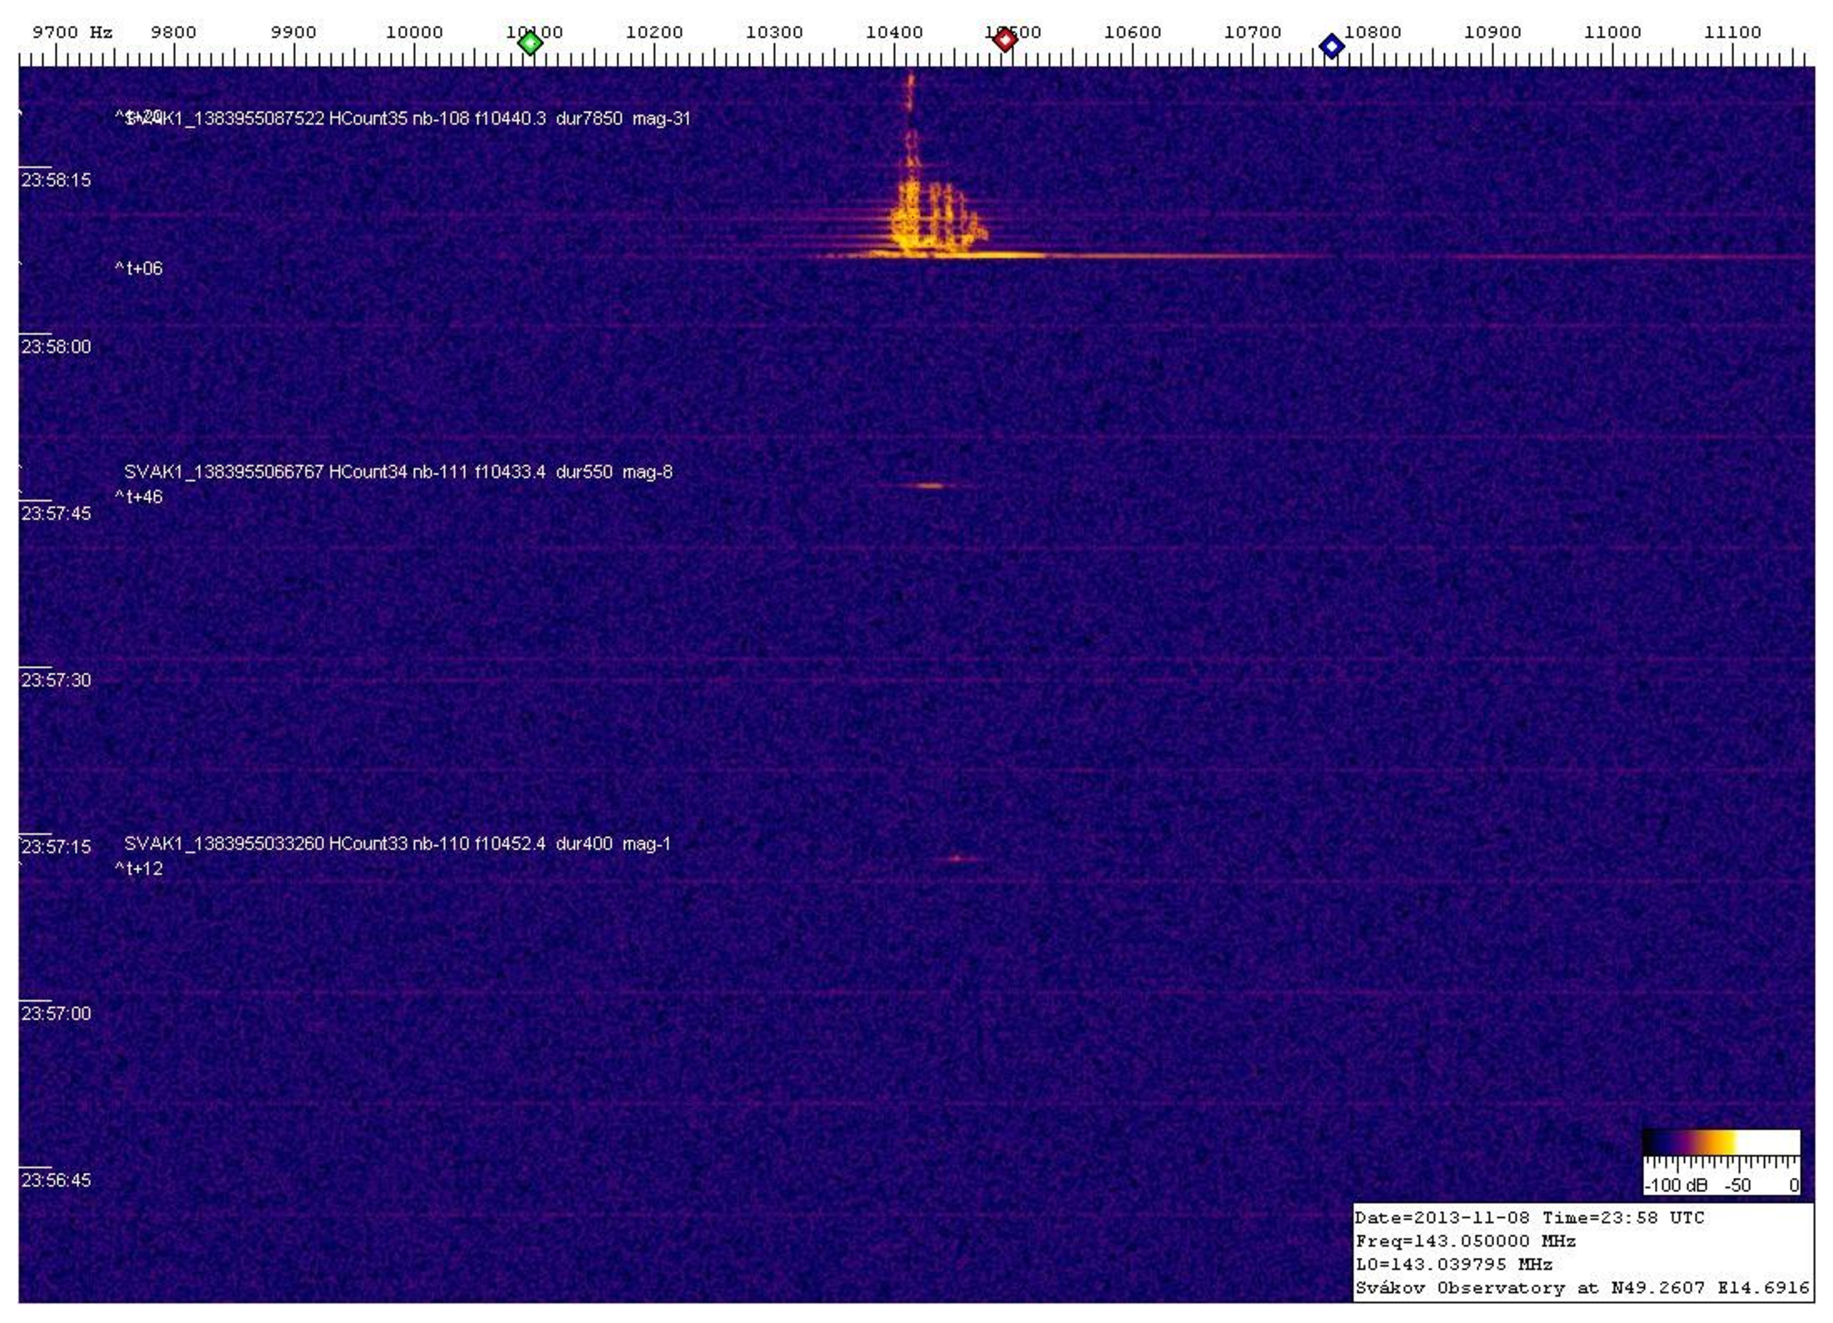
\includegraphics[width=9cm]{graves/graves_soubory/image007.eps}
	  	\caption{Záznam radiového bolidu.}
	  	\label{fig:}
	\end{center}
\end{figure}
Na uvedeném záznamu jsou nejdříve vidět dva drobné meteory v časech 23:57:12 a 23:57:46. Poté je nahoře větší meteor ve 23:58:06, u kterého je dobře patrný takzvaný čelní odraz (head echo). To je ta téměř vodorovná čára zprava, která vzniká Dopplerovským posuvem díky deceleraci meteoru. Změně frekvence 1 Hz odpovídá změna rychlosti cca 2 m/s. Poté je vidět odraz od stopy meteoru. Vlastně je zde vidět několik odrazů. Zřejmě došlo k rozpadu tělesa a vzniklo několik stop, které se rozpínají různou rychlostí a jsou v různých výškách unášeny prouděním v atmosféře. Vodorovné čáry přes celou šířku záznamu nejsou poruchy, ale jsou to přesné časové značky po deseti sekundách, které se přimíchávají na pokročilejší stanici RMDS01B do signálu. Tyto značky jsou odvozeny od časového normálu GPS přijímače a pomáhají nám porovnávat záznamy z více stanic.

Kromě meteorů ovšem můžete na záznamech najít i jiné věci. Například na Obr. 6 je vidět zánik druhého stupně nosné rakety Sojuz-U tak, jak ho zaznamenaly přijímače v Úpici, Praze a Českých Budějovicích. Možná si vzpomenete na tuto událost, která prošla tiskem, protože tento úkaz zpozorovali piloti dopravních letadel. Odraz od vlastního tělesa je ta šikmá čára, vertikální čára je opět odraz od ionizační stopy.
\begin{figure}[htbp]
	\begin{center}
		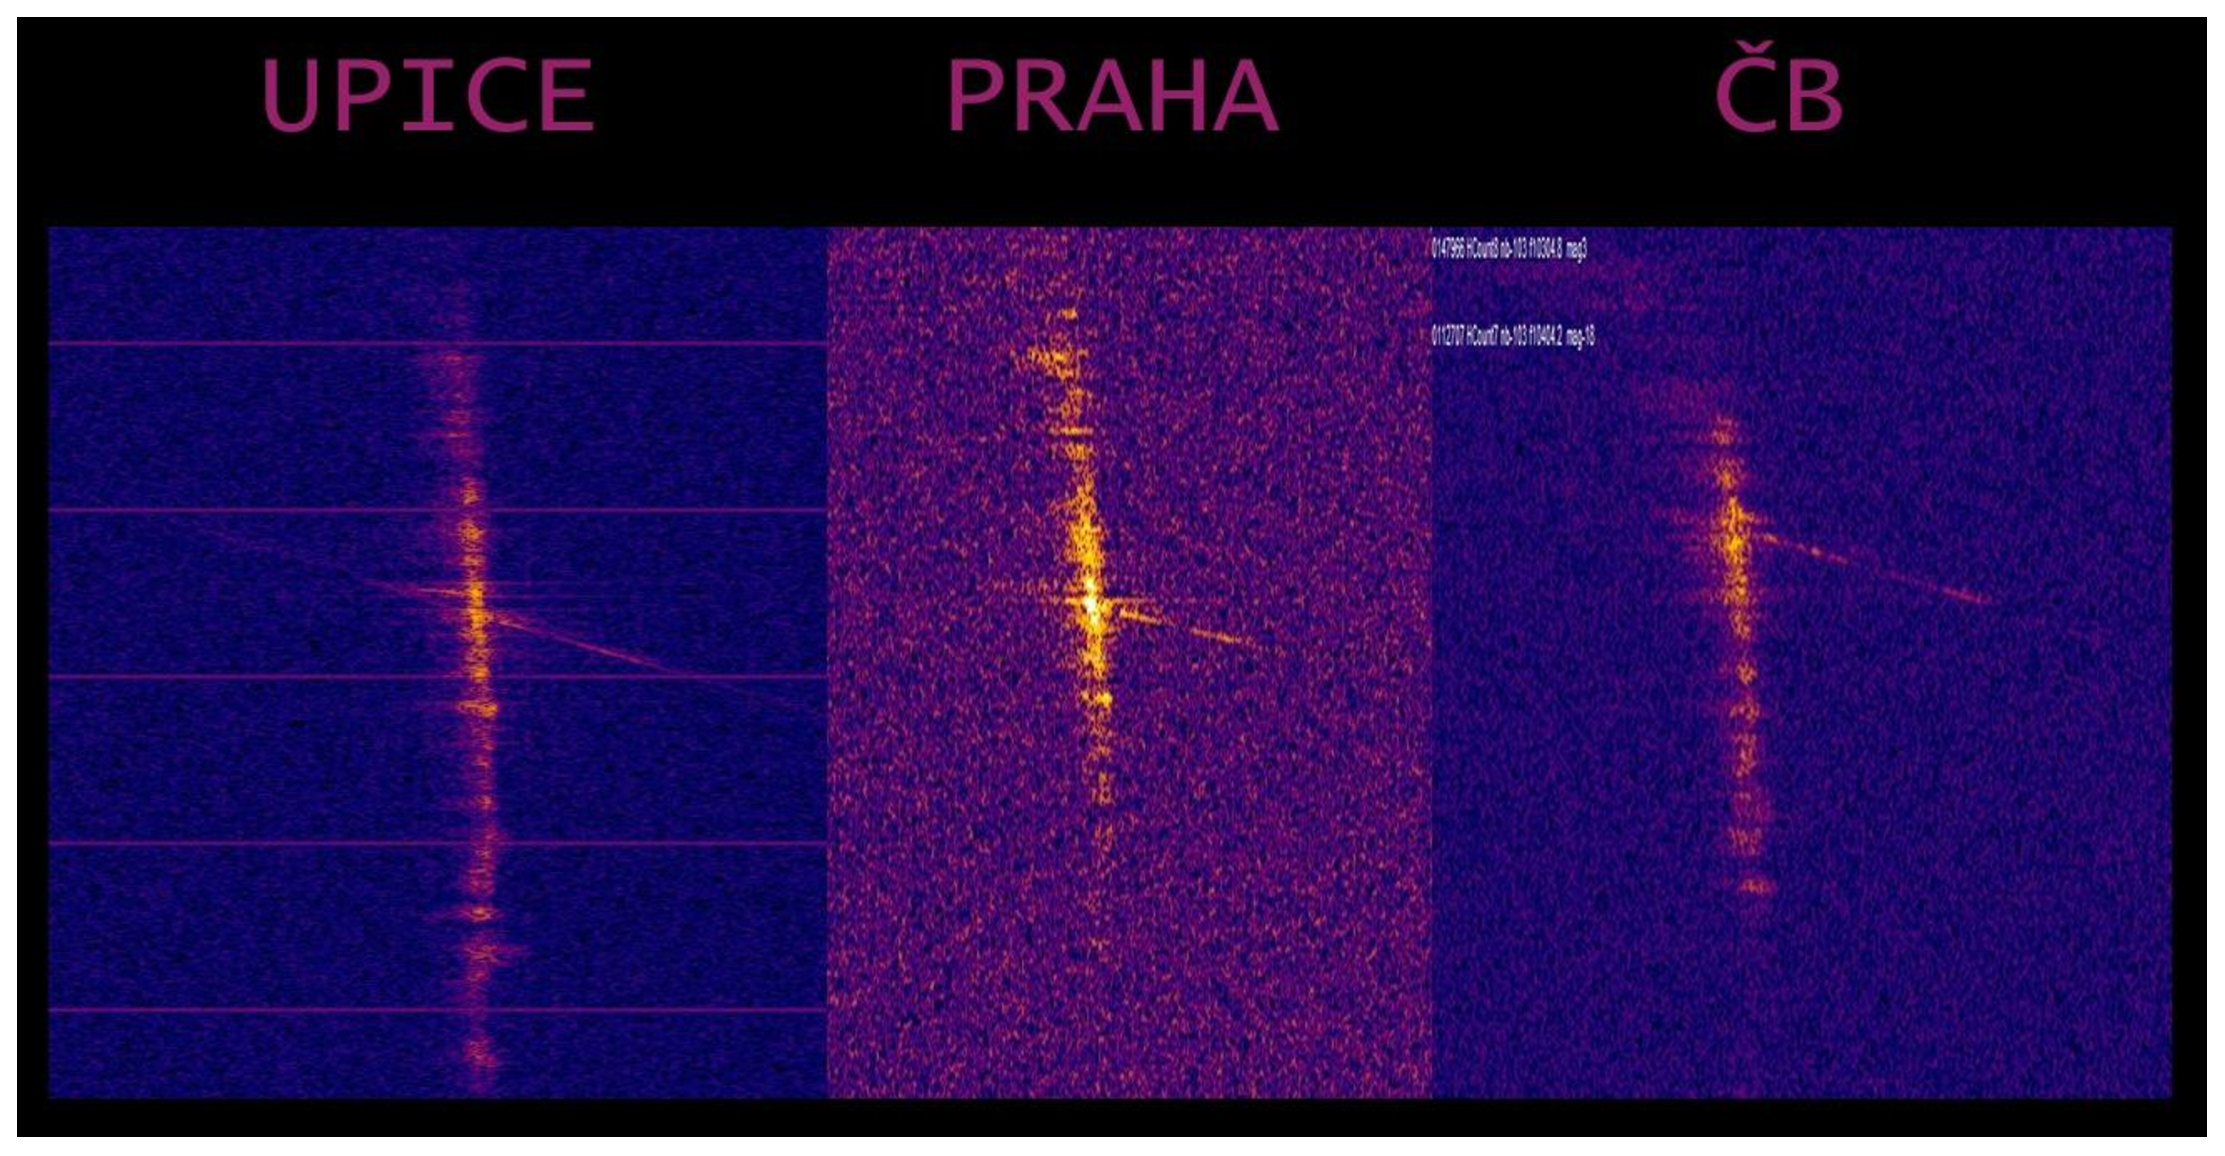
\includegraphics[width=9cm]{graves/graves_soubory/image008.eps}
	  	\caption{Zánik druhého stupně rakety Sojuz-U 13. února 2013.}
	  	\label{fig:}
	\end{center}
\end{figure}
Možná naleznete na záznamech i něco jiného, ale o tom až někdy příště. 
Na závěr uvedeme ještě jeden graf (Obr. 7), na kterém je vidět denní variace četnosti meteorů. Graf vznikl zprůměrováním hodinových četností detekovaných meteorů za jeden rok na jedné stanici. Na horizontální ose jsou vyneseny hodiny v UT. Na vertikální ose jsou průměrné počty meteorů za příslušnou hodinu. 
\begin{figure}[htbp]
	\begin{center}
		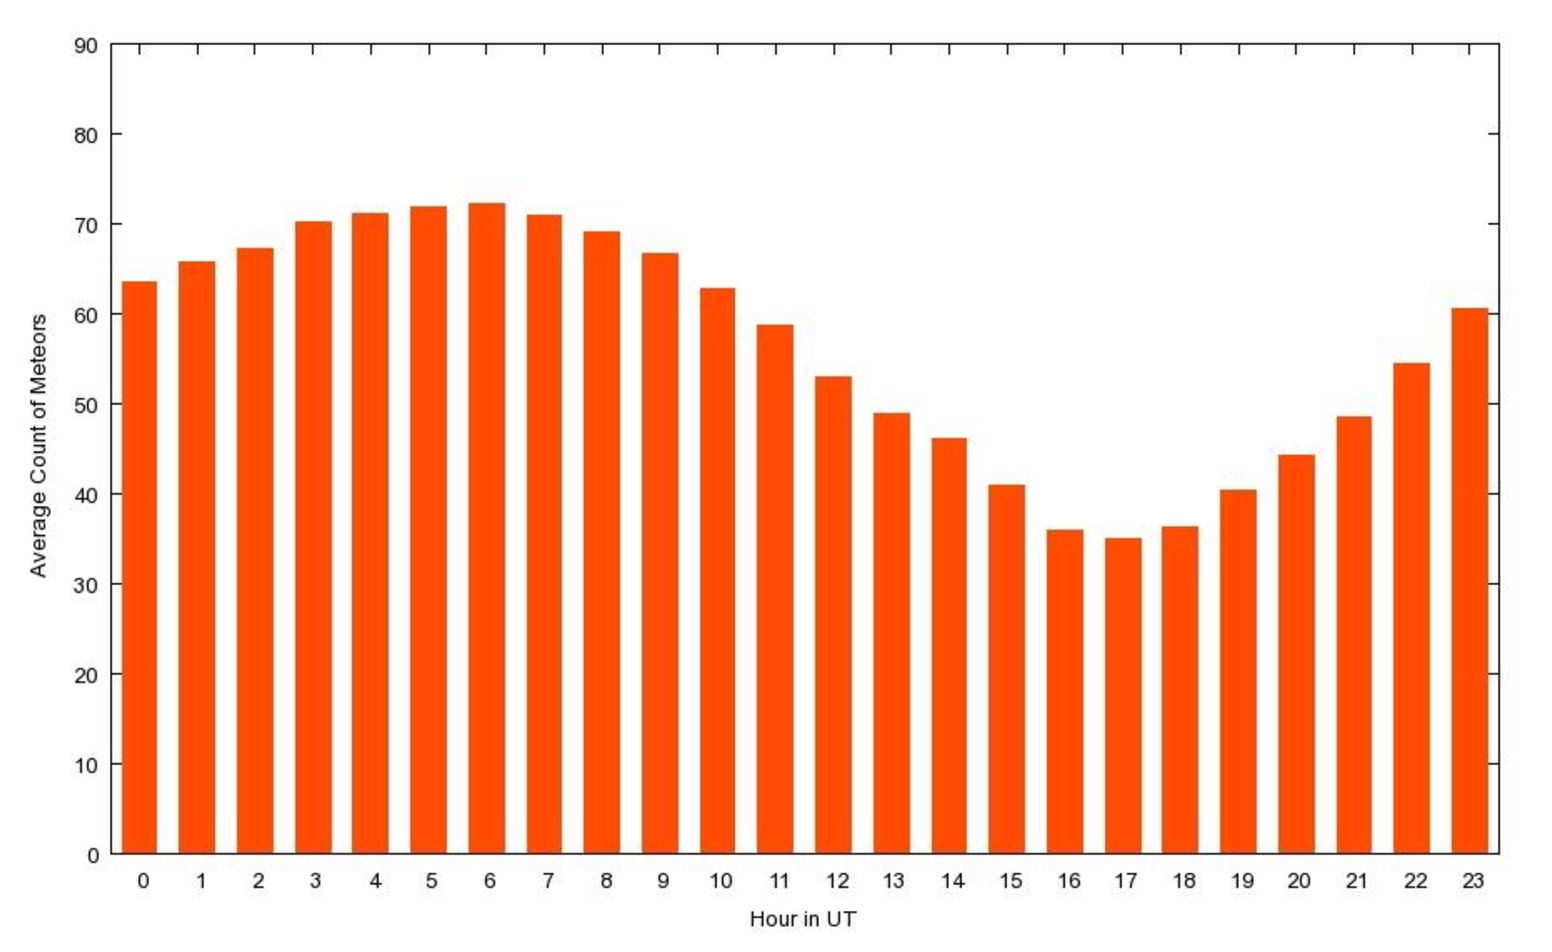
\includegraphics[width=9cm]{graves/graves_soubory/image009.eps}
	  	\caption{Průměrné hodinové četnosti meteorů naměřené na hvězdárně Svákov v období od září 2011 do srpna 2012.}
	  	\label{fig:}
	\end{center}
\end{figure}
Je vidět, že statisticky nejvíce meteorů padá mezi sedmou a osmou hodinou ranní středoevropského času, tedy v době, kdy již nelze meteory z našeho území pozorovat opticky, protože vychází Slunce, a to i v zimním období. V létě je samozřejmě situace ještě podstatně horší. Když si k tomu připočteme, že v polovině nocí svítí Měsíc, a že může být zataženo, lze opticky pozorovat pouze asi čtvrtinu meteorů z těch, které jsou pozorovatelné výše uvedenou metodou radiově. Z uvedeného grafu jasně vyplývá důležitost radiového pozorování, které je nezávislé na počasí a denní době.

\section*{Co dělám ve svojí hvězdárně?}
\autor{Vladimír Štefl}
Stojím a čumím! :-)

Ale teď vážně. Na nějakou vědeckou práci nemám samozřejmě uprostřed okresního města světelné (tmavé) podmínky. Zaměřuji se tedy na propagaci astronomie jako takové.
\begin{figure}[htbp]
 \centering
  \includegraphics*[width=11cm]{jezis/moon.eps}
\end{figure}

Ukazuji oblohu svým příbuzným a známým a samozřejmě dokládám patřičným výkladem.

Testuji okuláry a  příslušenství, které se snažím i vyrábět, což je celkem pochopitelné při dnešních cenách.
Momentálně začínám testovat cenově dostupné staré fotoobjektivy. Přikládám několik fotografií, pořízených fokálně za okulárem vlastní výroby; planety Jupiter, M 42 a Měsíce.

Světelné podmínky mám samozřejmě horšího charakteru, ale chci se pokusit i o snímky vzdálenějšího vesmíru. K fotografování používám t.z.v. bezzrcadlovku a chci samozřejmě zkusit i filmové aparáty (Zenit, Praktica a pod.).
\begin{figure}[htbp]
 \centering
  \includegraphics*[width=11cm]{jezis/star.eps}
\end{figure}
\begin{figure}[htbp]
 \centering
  \includegraphics*[width=6cm]{jezis/plan.eps}
\end{figure}

Pořídil jsem si i interferenčí filtry, které jsem už mnohokrát vyzkoušel při svých pozorováních. Jako nejlepší se zdají být UHC a OXYGEN III. Například mlhoviny se Střelci bez nich nejsou z města vůbec pozorovatelné! U M 42 s filtrem UHC doslova vyplují i okrajové filamenty. Při pozorování M 57 se dají použít filtry oba a s každým z nich je vidět něco jiného. Totéž platí u M 27 a dalších objektů. Jedině u galaxií a hvězdokup nepomohou, protože právě spektrum hvězd a rozptýleného světla potlačují. Peníze za interferenční filtry nejsou vůbec peníze vyhozené. Vřele doporučuji! 

Dále jsem zjistil, že ve městě, ale i na vesnici je vhodné použít dlouhou rosnici před objektivem (ale i u dalekohledu Newton), alespoň 2x delší, než je její průměr. Odstraní se tak boční světlo a nerosí se tak objektiv ano sekundární zrcátko u reflektorů.

Zkoušení různých doplňků dalekohledů a jejich kombinace se tak stává pomalu mojí doménou. Pakliže mi budou přát atmosférické podmínky, pokusím se příští číslo JihoČASu obohatit dalšími snímky a snad i novými poznatky z pozorování.


Večery takto strávené, bez televize, jsou mnohem lepší!

\section*{14. května 2014 uplynulo 20 let od „znovuotevření“ Hvězdárny F. Nušla při DDM v Jindřichově Hradci.}
\autor{Z jindřichohradecké Hvězdárny – Jana Jirků}

Než se tenkrát podařilo naši Hvězdárnu zachránit, nebyla ani Nušlova, ani pod Domem dětí a mládeže. Patřila městu J. Hradec a řídilo ji až do doby zavření (konec září 1992) Městské kulturní středisko. To bylo následně zrušeno pro svou – hmm, řekněme „neefektivitu“ :(, česky řečeno (a pochyceno tehdy od vcelku velmi důvěryhodných zdrojů), peníze a za peníze, za něž toto středisko mělo pro město něco dělat, nikdo a skoro nic a téměř nikdy neviděl. Po těch letech nechci rejpat, ale trochu mi to nesedí, když v téhle souvislosti vzpomenu, že každý konec roku jsem byla nucena sestavit jakýsi „rozpočet“ na rok další, který byl ale kompletně seškrtán, takže ve finále ho tvořit bylo stoprocentně zbytečné trápení a nezbylo pro nás ani na odbornou knížku. Moje námitky byly vždy odpálkovány \footnote{(budova Hvězdárny i pozemek kolem stále městu patří, a to je téměř bezplatně DDM pronajalo, ostatně stejně tak, jako v minulosti i Gymnáziu)} tvrzením, že knížek máme dost a když jsme namítali, že jsou staré a věda a výzkum jde dál, byli jsme poučeni, že fyzikální zákony se nemění! 

Naštěstí se ale vše v dobré obrátilo, Hvězdárna po potřebných jednáních, schváleních a úpravách začala sloužit opět svému účelu a slouží dál a věříme, že u toho i zůstane.

2. ledna 1994 proběhlo slavnostní předání Hvězdárny Gymnáziu Vítězslava Nováka v J. Hradci a tehdy nastala doba příprav na nové zahájení provozu. Rozebrané dalekohledy z kopule, do té doby z bezpečnostních důvodů uskladněné u mne doma, jsme museli sestavit a celou budovu uzpůsobit k dalšímu, novému fungování. Stihli jsme vše do 14. května 1994, který byl zároveň prvním „Dnem Astronomie“ nové éry Hvězdárny.

\begin{figure}[htbp]
 \centering
  \includegraphics*[width=10cm]{JH/hv.eps}
\end{figure}

Od roku 2000 jsme součástí Domu dětí a mládeže v J. Hradci. *  
I od té doby se mnoho změnilo k dobrému, ba i přímo skvělému, jen tak například uvedu: podařilo se nám Hvězdárnu pojmenovat po významném českém astronomovi, který se v Jindřichově Hradci narodil – Prof. Františku Nušlovi,  rozšířit arzenál astronomických dalekohledů o velmi dobré „kousky“ :), zjistili jsme, že 15. poledník nám vede hned před dveřmi do budovy Hvězdárny a podobně…

K dvacetiletému výročí jsme pořádali Výroční Den Astronomie a přednášku RNDr. Jiřího Grygara CSc. na téma „Od Tunguského meteoritu k Čeljabinsku aneb Země pod údery meteorické artilerie“.  Účast veřejnosti sice nebyla nijak valná, ale připisuji to špatnému, až hroznému počasí, které panovalo ten víkend, kdy se asi dobře sedí doma v teple a do té sloty se jednomu nechce vystrčit ani špičku nosu. 
\begin{figure}[htbp]
 \centering
  \includegraphics*[width=10cm]{JH/dale.eps}
\end{figure}
\begin{figure}[htbp]
 \centering
  \includegraphics*[width=10cm]{JH/moon.eps}
\end{figure}

Přestože jsme chystali páteční pozorování 16. května už od odpoledne do půlnoci, nic z toho nevyšlo, byla zima, zataženo a pršelo.
Snad ale už bude lépe, to si opravdu ze srdce přeju a myslím, nejen já.



\end{document}
 
 
%	\begin{itemize}
%	\item 
%	\end{itemize}
